\documentclass[conference]{IEEEtran}
\usepackage{times}
\usepackage[numbers,sort&compress]{natbib}
\usepackage{multicol}
\usepackage[bookmarks=true,hidelinks]{hyperref}
\usepackage{amsmath,amssymb,graphicx,booktabs}
\hypersetup{pdfauthor={},pdftitle={GPU-Accelerated Multibody Dynamics with Frictional Contact}}
\pagestyle{empty}
\newcommand{\norm}[1]{\left\lVert #1\right\rVert}
\makeatletter
\newenvironment{placedfigure}[1]{%
  \par\noindent\begin{minipage}{#1}\centering\def\@captype{figure}%
}{\end{minipage}\par\medskip}
\newenvironment{placedtable}{%
  \par\noindent\begin{minipage}{\columnwidth}\centering\def\@captype{table}%
}{\end{minipage}\par\medskip}
\makeatother

\begin{document}
\title{GPU-Accelerated Multibody Dynamics with Frictional Contact: A Differential Variational Inequality Solver for Robot Learning}
\author{Author Names Omitted for Anonymous Review}
\maketitle
\thispagestyle{empty}
\begin{abstract}
We describe Split Constraint Coupling (SCC), a GPU multibody solver integrated into Newton's Kamino simulator. SCC couples sparse joint factorization with projected iterations by alternating between blocks or taking a Schur complement. On two simulated closed-loop robots, Schur SCC gives \(10.3\)--\(136.4\times\) faster physics steps than dense-Cholesky proximal ADMM in 1,024 parallel environments at matched velocity-error limits. For frictional contact, we study nonlinear accelerated projected gradient descent (NAPGD), which evaluates the De Saxc\'e correction in every step. On a high-friction sliding box, NAPGD solves \(5.7\)--\(10.1\times\) faster than two other correction schedules at matched accuracy. Enabling the correction reduces the box's normal speed from 2.20 to below \(10^{-5}\) m/s. We train policies for robots with and without kinematic loops and demonstrate sim-to-real transfer on Unitree Go2, Unitree G1 with closed-loop ankle linkages, Disney Lanky Dog with closed-loop leg linkages, and Disney BDX.
\end{abstract}
\IEEEpeerreviewmaketitle

\section{Introduction}
Robot learning often runs thousands of simulations in parallel. Closed linkages couple bodies across several joints and can introduce redundant equations. The simulator must keep these loops closed while resolving changing contacts, joint limits, and motor forces. We use semi-implicit time stepping in maximal coordinates, with a pose and velocity for each body and the same equations for every joint~\citep{stewart}.

We describe Split Constraint Coupling (SCC), our GPU solver integrated into Newton's Kamino simulator~\citep{kamino,newton}. Kamino's proximal alternating direction method of multipliers (P-ADMM) solves joint and contact equations together in each update. Prior work has used projected GPU contact solvers and Schur complements for multibody contact~\citep{tasoragpu,mazhar,peiret}. A slip-dependent correction recovers the Coulomb friction law~\citep{acary,melanz,daviet,bogus}.
\begin{itemize}
\item A sparse GPU solver with two splitting methods. Alternating SCC solves each block in turn. Schur SCC includes the joint response in each projected step. Both apply the full constraint operator without assembling it.
\item A convergence comparison of both SCC methods and P-ADMM on saved walking states from Disney Research's DR Legs and Lanky Dog robots.
\item A sliding-box comparison of friction-correction schedules and a local convergence analysis for NAPGD.
\end{itemize}

\section{Split Constraint Coupling}
\subsection{One physics step}
A semi-implicit Euler step balances the change in body momentum against applied and constraint impulses,
\[
M(v^+-v)=h f_{\rm ext}+J^\top\lambda .
\]
Here \(h\) is the time step, \(M\) the mass matrix, \(f_{\rm ext}\) the applied loads, and \(J\) the constraint Jacobian. The free velocity is \(v_f=v+hM^{-1}f_{\rm ext}\). Applying \(M^{-1}\) to the body impulses \(J^\top\lambda\), then mapping to constraint space with \(J\), gives
\[
Jv^+ = \underbrace{Jv_f}_{\text{free velocity}}
    + \underbrace{(JM^{-1}J^\top)\lambda}_{\text{change due to impulses}} .
\]
The Delassus operator \(JM^{-1}J^\top\) maps impulses to changes in constraint velocity. We measure the mismatch from the target velocity \(v_{\rm tgt}\) as \(w=Jv^+-v_{\rm tgt}+R\lambda\), where \(R\lambda\) accounts for implicit drives and compliance. Joint equalities require \(w_b=0\). The other entries \(w_u\) enter the contact, joint-limit, and motor laws and can be nonzero. Substituting \(Jv^+\) gives
\begin{equation}
\begin{bmatrix}0\\w_u\end{bmatrix} =
\begin{bmatrix}B&F\\F^\top&U\end{bmatrix}
\begin{bmatrix}\lambda_b\\\lambda_u\end{bmatrix}+
\begin{bmatrix}b_b\\b_u\end{bmatrix}.
\label{eq:blocks}
\end{equation}
Here \(b=Jv_f-v_{\rm tgt}\), and \(B,F,U\) are blocks of \(JM^{-1}J^\top+R\). Joint impulses \(\lambda_b\) are free. The impulses \(\lambda_u\) obey the friction cones and joint-limit and motor-effort bounds.

\paragraph{Alternating SCC.} We factor the joint block once per time step. Each pass holds \(\lambda_u\) fixed while solving the joint equations, then updates \(\lambda_u\) with projected Gauss--Seidel (PGS) sweeps. The next joint solve responds to the new impulses.

\paragraph{Schur SCC.} Solving the joint equations for \(\lambda_b\) and substituting it into the remaining equations gives
\begin{equation}
 S=U-F^\top B^{-1}F,\qquad
 w_u=S\lambda_u+b_u-F^\top B^{-1}b_b .
\label{eq:schur}
\end{equation}
We apply \(B^{-1}\) with sparse Cholesky solves. The operator \(S\) includes the joint response in each projected update. Once \(\lambda_u\) is known, we recover \(\lambda_b=-B^{-1}(F\lambda_u+b_b)\). For exact block solves on a fixed linear active set, an alternating pass multiplies the impulse error by \(U^{-1}F^\top B^{-1}F\). Eigenvalues close to one explain why repeated passes can reduce the error slowly.

We apply \(JM^{-1}J^\top\) using sparse Jacobians and per-body mass blocks. We assemble \(B\) for Cholesky and can store small reduced blocks. A diagonal shift \(E\) stabilizes redundant joint equations. An exact solve with \(B+E\) leaves the defect \(-E\lambda_b\) in the original joint equations.

\clearpage
\twocolumn[{\begin{placedfigure}{\textwidth}
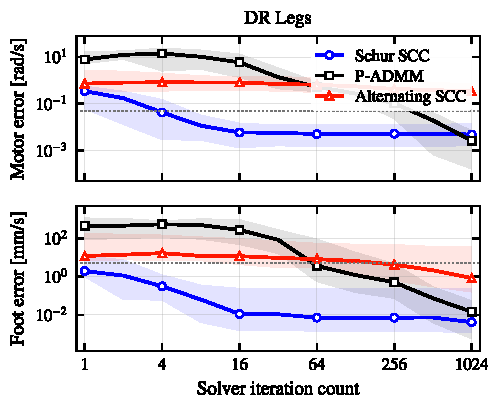
\includegraphics[width=.488\textwidth]{figures/walking_dr_legs.pdf}\hfill
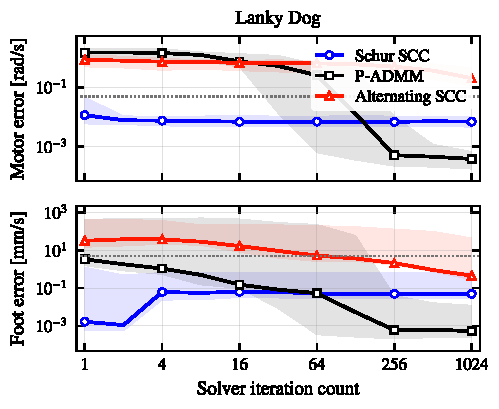
\includegraphics[width=.488\textwidth]{figures/walking_lanky_dog.pdf}
\caption{Joint and foot velocity errors across 44 saved walking states per robot. The curves show the median, and the shaded bands span the 10th to 90th percentiles. The reference uses a P-ADMM cap of 2,000 updates. An SCC iteration is one pass with ten PGS sweeps. A P-ADMM iteration includes one global solve, a projection, and a multiplier update. Dotted lines mark the error limits.}
\label{fig:walking}
\end{placedfigure}}]

\section{Accuracy and GPU Time on Walking States}
\paragraph{Policies and saved states.} We train one velocity-tracking policy per robot with 1,000 proximal policy optimization (PPO) updates in 4,096 environments. Each step uses four Schur SCC passes and ten PGS sweeps per pass. With fixed policies, we sample at regular intervals starting 2 s into each episode, yielding 11 snapshots of pose, velocity, motor commands, and contacts. Four episodes provide 44 snapshots to choose iteration budgets and the initial P-ADMM penalty. Four more provide 44 test snapshots. Both robots complete all test episodes. DR Legs averages \(0.103\) m/s at a command of \(0.20\) m/s, and Lanky Dog averages \(0.503\) m/s at \(0.50\) m/s.

Each solver takes one 4 ms step from the same snapshot, starting from zero impulses with position recovery disabled. DR Legs~\citep{gim} has six linkage loops, 180 joint equality rows, and 36--69 projected rows. Lanky Dog has four loops, 164 joint equality rows, and 31--39 projected rows.

\paragraph{Reference velocities.} For each test snapshot, we take a step with P-ADMM and use its result at a cap of 2,000 updates as the reference \(v_{\rm ref}\). Doubling the cap to 4,000 changes the foot-contact velocities by at most 0.12 mm/s and driven-joint speeds by at most 0.005 rad/s.

\paragraph{Velocity error limits.} We allow 10 mm/s for base translation, 0.02 rad/s for base rotation, 0.05 rad/s at every driven joint, and 5 mm/s along the ground at every foot contact. The whole-body error \(\sqrt{\Delta v^\top M\Delta v/m_{\rm robot}}\) must stay within 10 mm/s, where \(\Delta v=v^+-v_{\rm ref}\) and \(m_{\rm robot}\) is the total robot mass.

\paragraph{Error versus iteration count.} We run each solver for 1 to 1,024 iterations (Fig.~\ref{fig:walking}). On DR Legs, the fastest Schur SCC settings that meet the limits use 4 to 16 passes, depending on the snapshot. P-ADMM uses a median of 512 updates. On Lanky Dog, four Schur passes suffice for all 44 snapshots, and P-ADMM uses a median of 128 updates. Alternating SCC meets the limits on one snapshot per robot within the tested counts.

On these snapshots, Schur with PGS gives lower median joint and foot errors than accelerated projected gradient descent (APGD) with an outer friction-correction loop at comparable GPU solve times. At high PGS counts, the median joint error is close to that from solving the stabilized equations in double precision.

\begin{placedtable}
\caption{GPU time for one complete step across 1,024 parallel environments, in ms. Both solvers meet the velocity limits on all 44 test snapshots per robot.}
\label{tab:timing}
\begin{tabular}{@{}lrrrr@{}}
\toprule
Robot & States & Schur & P-ADMM & Ratio\\\midrule
DR Legs & 44/44 & 57.30 & 589.28 & \(10.3\times\)\\
Lanky Dog & 44/44 & 3.44 & 469.94 & \(136.4\times\)\\\bottomrule
\end{tabular}
\end{placedtable}
\paragraph{Batched step time.} We repeat the test snapshots across 1,024 parallel environments. Schur SCC uses 128 passes on DR Legs and four on Lanky Dog, with ten PGS sweeps per pass. P-ADMM uses preconditioned dense Cholesky solves and allows up to 1,024 updates, with an initial penalty of 0.1 for DR Legs and 0.01 for Lanky Dog. We check velocity accuracy on three repeats. Table~\ref{tab:timing} reports the median of 15 CUDA timings on an RTX PRO 4500 Blackwell, including collision detection, assembly, factorization, the solve, and integration. For Lanky Dog, eliminating 164 joint equations leaves at most 39 rows for the projected solve, which helps explain the speedup.

\paragraph{Hardware transfer.} We transfer policies trained in simulation to Unitree Go2, Unitree G1, Disney Lanky Dog, and Disney BDX. G1 has closed-loop ankle linkages, and Lanky Dog has closed-loop leg linkages. The Go2 policy was trained with a standalone predecessor of SCC and walks on rough outdoor terrain.

\clearpage
\twocolumn[{\begin{placedfigure}{\textwidth}
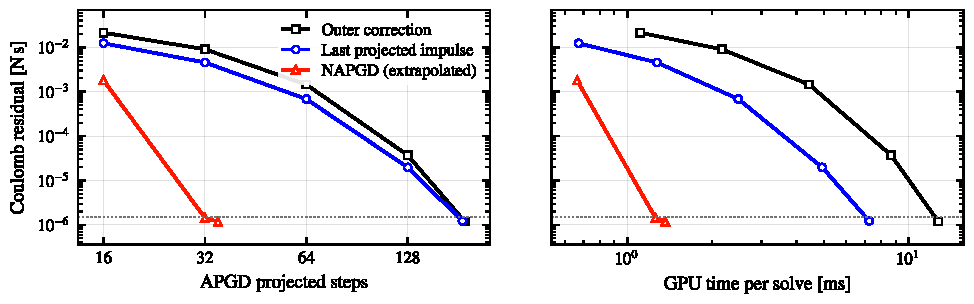
\includegraphics[width=.94\textwidth]{figures/contacts_sliding_box.pdf}
\caption{Three friction-correction schedules on a box sliding initially at 10 m/s with \(\mu=4\). NAPGD updates the correction at the extrapolated impulse. At each iteration cap, we plot the largest Coulomb residual across seven runs against the median step count and GPU contact-solve time. Dotted lines mark \(r_c=1.5\times10^{-6}\,\mathrm{N\,s}\).}
\label{fig:sliding}
\end{placedfigure}}]

\section{Nonlinear APGD for Sliding Contact}
\paragraph{Artificial separation.} Let \(x=(x_t,x_n)\) and \(v=(v_t,v_n)\) denote a contact impulse and its relative velocity. The friction cone \(K_\mu=\{x:x_n\geq0,\ \norm{x_t}_2\leq\mu x_n\}\) has dual \(K_\mu^*=\{z:z_n\geq\mu\norm{z_t}_2\}\). The uncorrected cone law enforces \(v\in K_\mu^*\) and \(x^\top v=0\). At a loaded contact, these conditions imply \(v_n=\mu\norm{v_t}_2\), so sliding creates artificial separation, or dilatancy.

The De Saxc\'e correction sets \(G=(v_t,v_n+\mu\norm{v_t}_2)\) and enforces \(G\in K_\mu^*\) and \(x^\top G=0\)~\citep{acary}. Dual feasibility now gives \(v_n\geq0\). Orthogonality gives
\[
0=x_n v_n+\underbrace{x_t^\top v_t+\mu x_n\norm{v_t}_2}_{\geq 0}.
\]
The bracket is nonnegative by the friction bound. Thus \(x_n v_n=0\), and a loaded contact has zero separating velocity even during slip.

\paragraph{Projected step.} Write \(v(x)=Ax+b\) and \(G(x)=v(x)+s(v(x))\), where \(s\) stacks the normal corrections. The Schur complement includes the joint response in \(A\). The outer-loop method holds \(s\) fixed for each APGD solve, updates it from the new impulse, and restarts acceleration. NAPGD evaluates the correction at the extrapolated impulse \(y_k=x_k+\beta_k(x_k-x_{k-1})\),
\begin{equation}
 x_{k+1}=\Pi_K\!\left(y_k-h_k
   [v(y_k)+s(v(y_k))]\right).
 \label{eq:apgd}
\end{equation}
A third variant evaluates the correction at \(x_k\) with the same \(v(y_k)\), restart, and line search. We measure the residual
\begin{equation}
 r_c(x)=\norm{x-\Pi_K\!\left(x-h_0G(x)\right)}_\infty,
 \label{eq:contact}
\end{equation}
where \(h_0=1\,\mathrm{kg}\) and \(\Pi_K\) projects onto the product \(K\) of the friction cones.

\paragraph{Sliding box.} A 1 kg box touches a plane at four corners and slides at 10 m/s with \(\mu=4\). After a \(1/60\) s step, NAPGD matches the analytical Coulomb slip speed of 9.346 m/s and keeps the normal speed below \(10^{-5}\) m/s at all corners. With the correction disabled, the solver gives 0.550 m/s of slip and 2.199 m/s of normal separation.

To reach \(r_c\leq1.5\times10^{-6}\,\mathrm{N\,s}\) and a contact velocity error of at most \(2\times10^{-5}\) m/s, NAPGD takes 32 steps and 1.26 ms. Updating the correction at \(x_k\) takes 186 steps and 7.24 ms (Fig.~\ref{fig:sliding}). Among the tested inner caps of 1, 4, 16, 64, and 256 steps, the fastest passing outer-loop setting uses one APGD step per cycle. It takes 189 cycles and 12.75 ms.

\paragraph{Existence and local convergence.} If \(A\succeq0\) and \(K\cap\ker A=\{0\}\), the Coulomb problem has a solution~\citep{acary}. On \(K\), \(x^\top A x\) grows quadratically and \(x^\top s(v(x))\geq0\), so \(x^\top G(x)>0\) at a large radius. Continuity gives a solution on the compact truncated cone. Testing at zero forces \(x^\top G(x)\leq0\), so the solution lies inside the sphere and solves the full problem.

For fixed \(h>0\), we analyze \(P_h(y)=\Pi_K(y-hG(y))\) near a solution with positive normal impulses and nonzero slip. We take the derivative along the active cone boundary. The update converges locally if that derivative has a real eigenbasis and all its eigenvalues lie in \((-1/3,1)\). For a mode with eigenvalue \(\gamma\), the linearized error satisfies
\begin{equation}
 e_{k+1}=\gamma[e_k+\beta_k(e_k-e_{k-1})].
\end{equation}
For \(0<\gamma<1\), the quantity \((1-\gamma)e_k^2+\gamma(e_k-e_{k-1})^2\) decreases by a factor of at most \(\gamma\) per step. For \(-1/3<\gamma<0\), the bound \(|e_{k+1}|\leq|\gamma|(2|e_k|+|e_{k-1}|)\) gives contraction in a weighted norm. Both bounds hold for \(\beta_k\in[0,1]\), including restarts. In a separate two-contact problem with a known solution, the residual stays above the tolerance at the iteration cap.

\section{Conclusion}
By including the joint response in each projected update, Schur SCC meets the same velocity-error limits as P-ADMM on saved walking states from both closed-loop robots, with lower GPU step times. In the sliding test, evaluating the De Saxc\'e correction at every accelerated step reaches the target accuracy faster than an outer correction loop and reproduces Coulomb sliding with negligible normal separation.

The final version will provide a fuller numerical analysis of convergence and velocity error, along with the training, deployment, and hardware evaluation details for the four sim-to-real demonstrations.

\clearpage
\begin{thebibliography}{11}
\bibitem[Stewart and Trinkle(1996)]{stewart}
D. E. Stewart and J. C. Trinkle.
An implicit time-stepping scheme for rigid body dynamics with inelastic collisions and Coulomb friction.
\emph{International Journal for Numerical Methods in Engineering}, 39(15):2673--2691, 1996.

\bibitem[Tsounis et~al.(2026)]{kamino}
V. Tsounis, G. Maloisel, C. Schumacher, R. Grandia, A. Serifi, D. M\"uller, C. Amevor, T. Widmer, and M. B\"acher.
Kamino: GPU-based simulation of rigid multi-body physics with kinematic loops.
\emph{arXiv:2603.16536v2}, 2026.

\bibitem[Newton Physics Contributors(2026)]{newton}
Newton Physics Contributors.
\emph{Newton Physics Engine}. Software revision \texttt{7a23bbd01dfd}, 2026.

\bibitem[Mazhar et~al.(2015)]{mazhar}
H. Mazhar, T. Heyn, D. Negrut, and A. Tasora.
Using Nesterov's method to accelerate multibody dynamics with friction and contact.
\emph{ACM Transactions on Graphics}, 34(3), Article 32, 2015.

\bibitem[Melanz et~al.(2016)]{melanz}
D. Melanz, H. Mazhar, and D. Negrut.
Using an anti-relaxation step to improve the accuracy of the frictional contact solution in a DVI framework for rigid body dynamics.
\emph{ASME International Design Engineering Technical Conferences}, 2016. DOI 10.1115/DETC2016-59651.

\bibitem[Acary et~al.(2011)]{acary}
V. Acary, F. Cadoux, C. Lemar\'echal, and J. Malick.
A formulation of the linear discrete Coulomb friction problem via convex optimization.
\emph{ZAMM}, 91(2):155--175, 2011.

\bibitem[Daviet et~al.(2011)]{daviet}
G. Daviet, F. Bertails-Descoubes, and L. Boissieux.
A hybrid iterative solver for robustly capturing Coulomb friction in hair dynamics.
\emph{ACM Transactions on Graphics}, 30(6), Article 139, 2011.

\bibitem[Daviet()]{bogus}
G. Daviet.
\emph{So-Bogus: A Sparse, Optimization-Based, GPL Unilateral Solver}. Projected-gradient solver implementation, software revision \texttt{bc670d9305fa}.

\bibitem[Tasora et~al.(2011)]{tasoragpu}
A. Tasora, D. Negrut, and M. Anitescu.
GPU-based parallel computing for the simulation of complex multibody systems with unilateral and bilateral constraints.
In \emph{Multibody Dynamics}, pages 283--307. Springer, 2011.

\bibitem[Peiret et~al.(2019)]{peiret}
A. Peiret, S. Andrews, J. K\"ovecses, P. G. Kry, and M. Teichmann.
Schur complement-based substructuring of stiff multibody systems with contact.
\emph{ACM Transactions on Graphics}, 38(5), Article 150, 2019.

\bibitem[Gim et~al.(2018)]{gim}
K. G. Gim, J. Kim, and K. Yamane.
Design and fabrication of a bipedal robot using serial-parallel hybrid leg mechanism.
In \emph{IEEE/RSJ International Conference on Intelligent Robots and Systems}, 2018. DOI 10.1109/IROS.2018.8594182.
\end{thebibliography}

\end{document}
